\documentclass[11pt,a4paper]{article}

\usepackage{epsfig}
\usepackage{multicol}

\usepackage[utf8]{inputenc}
\usepackage[brazil]{babel}
\usepackage{fancyheadings}
\usepackage{amsmath}
\usepackage{calrsfs}
\usepackage{enumerate}
\usepackage{enumitem}   
\DeclareGraphicsExtensions{.png,.pdf}
\usepackage{amsmath, amsfonts, amssymb}
\usepackage{esint}
\usepackage{graphicx}
\usepackage{multicol}
\usepackage{tasks}
\usepackage[utf8]{inputenc}
\usepackage{mathrsfs} % Transformada de Laplace
\usepackage{indentfirst}
\usepackage{xcolor}

% As margens
\setlength{\textheight}{24.0cm}
\setlength{\textwidth}{17.5cm}
\setlength{\oddsidemargin}{2.0cm} % Margens reais desejadas
\setlength{\evensidemargin}{2.0cm} % 2+17.5+1.5=21cm (largura A4)
\setlength{\topmargin}{1.5cm} % 1.5+1.6+1.0+24.0+1.6=29.7cm
\setlength{\headheight}{1.6cm} % (altura A4)
\setlength{\headsep}{1.0cm}
\setlength{\columnsep}{1.5cm} % Coluna = 8cm ((17.5-1.5)/2)
\addtolength{\oddsidemargin}{-1in}
\addtolength{\evensidemargin}{-1in}
\addtolength{\topmargin}{-1in}
\setlength{\footskip}{0.0cm}


% Novos comandos
\newcommand{\limite}{\displaystyle\lim}
\newcommand{\integral}{\displaystyle\int}
\newcommand{\somatorio}{\displaystyle\sum}
\newcommand{\mat}[1]{\mbox{\boldmath{$#1$}}} 

\pagestyle{fancy}


\usepackage{lipsum}

\lhead{

\includegraphics[width=1cm]{brasao.png}
}

\rhead{ 
\sc\textbf{U}niversidade \textbf{F}ederal do \textbf{C}eará\\
Campus Quixadá\\ Lista 2 de Eletromagnetismo}

\cfoot{}

\begin{document}

	\begin{center}
		\Large Eletrostática - Lei de Gauss. 
	\end{center}

\begin{flushleft}
\textbf{Nome:} Mateus Sousa Araújo. \\
\textbf{Matrícula:} 374858. \\
\textbf{Professor:} Antônio Joel Ramiro de Castro. \\
\textbf{Curso:} Engenharia de Computação. \\
\end{flushleft}

\begin{enumerate}

\item \textbf{Griffiths - Cap. 2 - Problema 2.12.}

Use a Lei de Gauss para encontrar o campo elétrico dentro de uma esfera uniformemente carregada (com densidade de carga $\rho$). 

\textbf{RESOLUÇÃO}

\begin{figure}[h]	
\centering % para centralizarmos a figura	
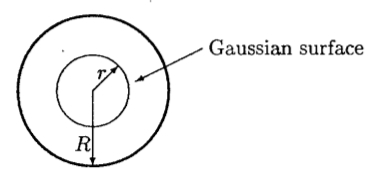
\includegraphics[width=6cm]{Selection_077.jpg} 
\caption{Superfície Gaussiana em uma esfera.}
\end{figure}

Precisamos considerar que o campo gerado por essa esfera é constante em toda sua redondeza. Também precisamos adotar a densidade superficial de cargas na esfera e substituir na relação. Dessa forma, podemos escrever:

\begin{center}
$\displaystyle\oint \vec{E} \cdot \vec{da} = E \cdot 4\pi r^2 = \displaystyle\dfrac{Q_{int}}{\epsilon_0} $
\end{center}

\begin{center}
$E \cdot 4\pi r^2 = \displaystyle\dfrac{1}{\epsilon_0} \displaystyle\dfrac{4\pi r^3 \rho}{3} $
\end{center}

\begin{center}
$\vec{E} = \displaystyle\dfrac{1}{3\epsilon_0} \rho r \ \mat{\hat{r}} $
\end{center}

\item \textbf{Griffiths - Cap. 2 - Problema 2.13.}

Encontre o campo elétrico a uma distância $s$ de um fio reto de comprimento infinito, que tem uma densidade linear de carga uniforme $\lambda$. 

\textbf{RESOLUÇÃO}

\begin{figure}[h]	
\centering % para centralizarmos a figura	
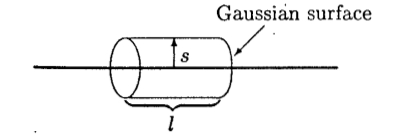
\includegraphics[width=6cm]{Selection_078.jpg} 
\caption{Superfície Gaussiana em um fio.}
\end{figure}

Primeiramente precisamos considerar que o campo gerado a uma distância $s$ do fio é sempre constante. Dessa forma, considerando a densidade linear e uma Gaussiana envolvendo o fio, temos:

\begin{center}
$\displaystyle\oint \vec{E} \cdot \vec{da} = E \cdot 2\pi s \cdot l = \displaystyle\dfrac{Q_{int}}{\epsilon_0} $
\end{center}

\begin{center}
$E \cdot 2\pi s \cdot l = \displaystyle\dfrac{\lambda l}{\epsilon_0} $
\end{center}

\begin{center}
$\vec{E} = \displaystyle\dfrac{\lambda}{2\pi \epsilon_0 s} \ \mat{\hat{s}} $
\end{center}

\item \textbf{Griffiths - Cap. 2 - Problema 2.19.}

Calcule $\vec{\nabla} \times \vec{E}$ ou $\displaystyle\oint \vec{E} \cdot \vec{dl} = 0$. Considere o campo elétrico gerado por uma carga pontual. 


\textbf{RESOLUÇÃO}

Considere um corpo extenso de densidade volumétrica $\rho$ que exerce um campo elétrico em um ponto P no espaço. Se tomarmos um ponto de origem O e fizermos os vetores de posição até o ponto P e calcularmos o campo elétrico, temos:

\begin{center}
$\vec{\nabla} \times \vec{E} = \displaystyle\dfrac{1}{4 \pi \epsilon_0} \displaystyle\int \rho (r')dv'\ \vec{\nabla} \times \left(\displaystyle\dfrac{\vec{r} - \vec{r'}}{|\vec{r} - \vec{r'}|^3}\right) $
\end{center}

Perceba que a variável em questão nesse caso é $r'$ pois esse vetor de posição é onde o corpo extenso se encontra com suas densidades de cargas infinitesimais. Logo, precisamos nos preocupar do operador nabla aplicado no versor unitário. Esse vetor unitário possui, em coordenadas cartesianas, a seguinte relação:

\begin{center}
$\displaystyle\dfrac{\vec{r} - \vec{r'}}{|\vec{r} - \vec{r'}|^3} = \displaystyle\dfrac{(x - x')\mat{\hat{i}} + (y - y')\mat{\hat{j}} + (z - z')\mat{\hat{k}}}{[(x - x')^2 + (y - y')^2 + (z - z')^2]^{3/2}}$
\end{center}

O operador nabla aplicado no versor fica da seguinte forma: 

\begin{center}
$\vec{\nabla} \times \left(\displaystyle\dfrac{\vec{r} - \vec{r'}}{|\vec{r} - \vec{r'}|^3}\right) = \left| \begin{array}{ccc}
\mat{\hat{i}} & \mat{\hat{j}}  & \mat{\hat{k}} \\ 
 \displaystyle\dfrac{\partial}{\partial x} & \displaystyle\dfrac{\partial}{\partial y} & \displaystyle\dfrac{\partial}{\partial z}\\
 \displaystyle\dfrac{(x - x')}{r^3} & \displaystyle\dfrac{(y - y')}{r^3}  & \displaystyle\dfrac{(z - z')}{r^3}
\end{array} \right|$

\end{center}

Fazendo o cálculo do determinante para o versor $\mat{\hat{i}}$, temos:

\begin{center}
$\mat{\hat{i}} \left[\displaystyle\dfrac{\partial}{\partial y} \displaystyle\dfrac{(z - z')}{r^3} - \displaystyle\dfrac{\partial}{\partial z} \displaystyle\dfrac{(y - y')}{r^3} \right] = 0$
\end{center}

Percebe-se que, para o versor $\mat{\hat{i}}$, o vetor nessa coordenada possui uma componente igual a zero. Isso também é perceptível para os outros versores. Podemos concluir então que o campo elétrico gerado por uma carga pontual é igual a zero. Se retornarmos à nossa integral de campo, a mesma dará zero também devido ao cálculo do rotacional do campo. 

Por propriedade, se o rotacional de um campo vetorial for igual a zero, dizemos que esse campo é conservativo. Se tomarmos a integral de linha deste campo em um contorno fechado, essa integral claramente será igual a zero devido à sua propriedade conservativa. A essa propriedade, chamamos de propriedade das integrais de linha, logo: 

\begin{center}
$\displaystyle\oint \vec{E} \cdot \vec{dl} = 0$
\end{center}

Concluindo assim que o campo elétrico gerado por cargas pontuais é de natureza conservativa.

\end{enumerate}
	
\end{document}